\documentclass[journal,12pt,twocolumn]{IEEEtran}
\IEEEoverridecommandlockouts
\usepackage{cite}
\usepackage{amsmath,amssymb,amsfonts,bm}
\usepackage{mathtools}
\usepackage{tkz-euclide} 
\usepackage{tikz}
\usetikzlibrary{calc,math}
 \usepackage{caption}
\usepackage{listings}
\usepackage{gensymb}
\let\vec\mathbf
\numberwithin{equation}{subsection}

\newcommand{\myvec}[1]{\ensuremath{\begin{pmatrix}#1\end{pmatrix}}}
\newcommand{\norm}[1]{\left\lVert#1\right\rVert}

\renewcommand\thesection{\arabic{section}}
\renewcommand\thesubsection{\thesection.\arabic{subsection}}
\renewcommand\thesubsubsection{\thesubsection.\arabic{subsubsection}}

\renewcommand\thesectiondis{\arabic{section}}
\renewcommand\thesubsectiondis{\thesectiondis.\arabic{subsection}}
\renewcommand\thesubsubsectiondis{\thesubsectiondis.\arabic{subsubsection}}
%\renewcommand{\theequation}{\theenumi}
%\numberwithin{equation}{enumi}

\providecommand{\mbf}{\mathbf}
\providecommand{\pr}[1]{\ensuremath{\Pr\left(#1\right)}}
\providecommand{\qfunc}[1]{\ensuremath{Q\left(#1\right)}}
\providecommand{\sbrak}[1]{\ensuremath{{}\left[#1\right]}}
\providecommand{\lsbrak}[1]{\ensuremath{{}\left[#1\right.}}
\providecommand{\rsbrak}[1]{\ensuremath{{}\left.#1\right]}}
\providecommand{\brak}[1]{\ensuremath{\left(#1\right)}}
\providecommand{\lbrak}[1]{\ensuremath{\left(#1\right.}}
\providecommand{\rbrak}[1]{\ensuremath{\left.#1\right)}}
\providecommand{\cbrak}[1]{\ensuremath{\left\{#1\right\}}}
\providecommand{\lcbrak}[1]{\ensuremath{\left\{#1\right.}}
\providecommand{\rcbrak}[1]{\ensuremath{\left.#1\right\}}}

\lstset{
frame=single, 
breaklines=true,
columns=fullflexible
}

\begin{document}

\title{Matrix Theory EE5609 - Assignment 5\\
}

\author{\IEEEauthorblockN{Sandhya Addetla}\\
\IEEEauthorblockA{PhD Artificial Inteligence Department} \\
AI20RESCH14001\\
 }

\maketitle
\begin{abstract}
 Find the asymptotes of the given hyperbola and also the equation to its conjugate hyperbola
\end{abstract}

Download all python codes from 
\begin{lstlisting}
https://github.com/SANDHYA-A/Assignment5/blob/master/Assignment5.py
\end{lstlisting}

\section{Problem Statement}
 Find the asymptotes of the given hyperbola and also the equation to its conjugate hyperbola
\begin{align}
19x^2 + 24xy+y^2-22x-6y=0 \label{1.1}
\end{align}
\section{Solution}
The general equation of second degree is given by
\begin{align}
ax^2+2bxy+cy^2+2dx+2ey+f=0\label{2.1}
\end{align}
and can be expressed as
\begin{align}
\vec{x}^T\vec{V}\vec{x}+2\vec{u}^T\vec{x}+f=0 \label{2.2}
\end{align}
where
\begin{align}
\vec{V} &= \vec{V}^T = \myvec{a & b \\ b & c}
\\
\vec{u} &= \myvec{d & e}
\intertext{Comparing equations \ref{1.1} and \ref{2.2} we get}
    \vec{V}=\vec{V}^T&=\myvec{19 & 12 \\ 12 &1}\label{2.5}\\
    \vec{u}&=\myvec{-11 \\-3 }\label{2.6}\\
    f&=0\label{2.7}
\end{align}   
Expanding the Determinant of $\vec{V}$.
\begin{align}
    \Delta_{V} &= \begin{array}{|cc|}
19 &12\\12 & 1
\end{array}<0\label{2.8}
\end{align}
Hence from \ref{2.8} given
equation represents the hyperbola.\\
The characteristic equation of $\vec{V}$ is obtained by evaluating the determinant 
\begin{align}
       \begin{array}{|c|}
V-\lambda\vec{I}
\end{array}&=0\\
   \begin{array}{|cc|}
19-\lambda & 12 \\ 12 & 1-\lambda
\end{array}&=0\\
    \brak{19-\lambda}\brak{1-\lambda}-144=0\\
    \lambda_{1}=-5,   \lambda_{2}= 25 \label{2.12}
\end{align}
The eigenvector $\vec{p}$ is defined as 
\begin{align}
    \vec{V}\vec{p}&=\lambda\vec{p}\\
    \implies (\vec{V}-\lambda\vec{I})\vec{p}&=0\label{2.14}
\end{align}
For $\lambda_1=-5$ ,
\begin{align}
    (\vec{V}-\lambda_1\vec{I})=\myvec{19+5 & 12 \\12 & 1+5}
\end{align}
By row reduction , 
\begin{align}
    &\myvec{24 & 12 \\12 & 6}\\
&\xleftrightarrow{R_2\leftarrow 2R_2 -R_1}
    \myvec{24 & 12 \\ 0& 0}\\
        &\xleftrightarrow{R_1\leftarrow \frac{R_1}{12}}
    \myvec{2 & 1 \\ 0& 0}
    \label{2.18}
\end{align}
Subsituting equation \ref{2.18} in equation \ref{2.14} we get
\begin{align}
        &   \myvec{2 & 1 \\ 0& 0}\myvec{v_1 \\ v_2}=\myvec{0 \\ 0}\label{2.19}
\end{align}
Where, $\vec{p}=\myvec{v_1\\v_2}$
Let $v_1=t$
\begin{align}
    v_2&=-2t
\end{align}
Eigen vector $\vec{p_1}$ is given by
\begin{align}
    \vec{p_1}&=\myvec{t \\ -2t}
\end{align}
Let $t=1$, we get
\begin{align}
        \vec{p_1}&=\myvec{1 \\-1 }\label{2.22}
\end{align}
For $\lambda_2=25$ ,
\begin{align}
    (\vec{V}-\lambda_2\vec{I})=\myvec{19-25 & 12 \\12 & 1-25}
\end{align}
By row reduction , 
\begin{align}
    &\myvec{-6 & 12 \\12 & -24}\\
&\xleftrightarrow{R_2\leftarrow R_2 +2R_1}
    \myvec{-6 & 12 \\ 0& 0}\\
        &\xleftrightarrow{R_1\leftarrow \frac{R_1}{6}}
    \myvec{-1 & 2 \\ 0& 0}
    \label{2.26}
\end{align}
Subsituting equation \ref{2.26} in equation \ref{2.14} we get
\begin{align}
        &   \myvec{-1 & 2 \\ 0& 0}\myvec{v_1 \\ v_2}=\myvec{0 \\ 0}\label{2.27}
\end{align}
Where, $\vec{p}=\myvec{v_1\\v_2}$
Let $v_1=t$
\begin{align}
    v_2&=\frac{t}{2}
\end{align}
Eigen vector $\vec{p_2}$ is given by
\begin{align}
    \vec{p_2}&=\myvec{t \\ \frac{t}{2}}
\end{align}
Let $t=1$, we get
\begin{align}
        \vec{p_2}&=\myvec{1 \\\frac{1 }{2}}\label{2.30}
\end{align}
By eigen decompostion $\vec{V}$ can be represented by
\begin{align}
    \vec{V}&=\vec{P}\vec{D}\vec{P}^T\label{2.31}
\end{align}
where 
\begin{align}
        \vec{P}&=\myvec{\vec{p_1} & \vec{p_2}}\label{2.32}\\
    \vec{D}&=\myvec{\lambda_1 & 0 \\0 & \lambda_2}\label{2.33}
\end{align}

Substituting equations \ref{2.22}, \ref{2.30} in equation \ref{2.32} we get 
\begin{align}
    \vec{P}&=\myvec{1 & 1 \\-1 & \frac{1}{2}}\label{2.34}
\end{align}
Substituting equation \ref{2.12} in \ref{2.33} we get
\begin{align}
       \vec{D}&=\myvec{-5 & 0\\0 & 25}\label{2.35}
\end{align}
Centre of the hyperbola is given by 
\begin{align}
    \vec{c}&=-\vec{V}^{-1}\vec{u}\\
    \implies\vec{c}&=-\frac{1}{125}\myvec{1&-12\\-12&19}\myvec{-11 \\ -3}\\
    \implies\vec{c}&=-\frac{1}{125}\myvec{25\\ 75}\\
    \implies\vec{c}&=\myvec{\frac{-1}{5}\\-\frac{3}{5}}
\end{align}
Since,
\begin{align}
    \vec{u}^T\vec{V}^{-1}\vec{u}-f = -4 < 0\label{2.40}
\end{align} 
we need to swap axes. In hyperbola,
\begin{align}
axes=
\begin{cases}
\sqrt{\frac{\vec{u}^T\vec{V}^{-1}\vec{u}-f}{\lambda_1}}\\ \sqrt{\frac{f-\vec{u}^T\vec{V}^{-1}\vec{u}}{\lambda_2}}
\end{cases}
\end{align}
From above equations we can say that,
\begin{align}
\sqrt{\frac{\vec{u}^T\vec{V}^{-1}\vec{u}-f}{\lambda_1}}=\sqrt{ \frac{4}{5}}\\
\sqrt{\frac{f-\vec{u}^T\vec{V}^{-1}\vec{u}}{\lambda_2}}=\sqrt{ \frac{4}{25}}
\end{align}
Now we have,
\begin{align}
    \vec{y}^T\vec{D}\vec{y}&=\vec{u}^T\vec{V}^{-1}\vec{u}-f \label{2.44}
\end{align}
where ,
\begin{align}
    \vec{y}&=\vec{P}^T(\vec{x}-\vec{c})
\end{align}
To get $\vec{y}$,
\begin{align}
\vec{y}&=\vec{P}^T\vec{x}-\vec{P}^T\vec{c}\\
    \vec{y}&= \myvec{1 & -1 \\ 1 & \frac{1}{2}}\vec{x}-\myvec{1 & -1 \\ 1 & \frac{1}{2}}\myvec{-\frac{1}{5}\\-\frac{3}{5}}\\
    \vec{y}&=\myvec{1 & -1 \\ 1 & \frac{1}{2}}\vec{x}-\myvec{\frac{2}{5}\\ -\frac{1}{2}}
\end{align}
Subsituting the equation \ref{2.35} in equation \ref{2.44}
\begin{align}
   \implies\vec{y}^T\myvec{-5 & 0 \\0 & 25}\vec{y}&= -4\label{2.49}
\end{align}
\ref{2.49} is the equation of the hyperbola. Equation of a hyperbola and the combined equation of the Asymptotes differ only in the constant term.
\begin{align}
 19x^2 + 24xy+y^2-22x-6y+K=0   
\end{align}
The above equation can be expressed in the form 
\begin{align}
\vec{x}^T\vec{V}\vec{x}+2\vec{u}^T\vec{x}+f&=0 \label{2.51}
\intertext{Comparing equation we get}
    \vec{V}=\vec{V}^T&=\myvec{19 & 12 \\ 12 &1}\label{2.52}\\
    \vec{u}&=\myvec{-11 \\-3 }\label{2.53}\\
    f&=K\label{2.54}
\end{align}
\begin{align}
\Delta&=\begin{array}{|ccc|}19 & 12 & -11\\ 12& 1 & -3\\ -11 & -3 & K
\end{array}
\end{align}
Since the equations represent pair of straight lines, equating the determinant to zero, we can get the value of K
\begin{align}
\implies K=4
\end{align}
Let the equations of lines be,
\begin{multline}
	\brak{\vec{n_1}^T \vec{x} - c_1}\brak{\vec{n_2}^T \vec{x} - c_2} =\\
        \vec{x}^{T}\vec{Vx} + 2\vec{u}^{T}\vec{x} + f=0\label{2.57}
\end{multline}
\begin{multline}
\brak{\vec{n_1}^T\vec{x}-c_1}\brak{\vec{n_2}^T\vec{x}-c_2}=\\ \vec{x}^T\myvec{19 & 12 \\ 12 & 1}\vec{x}+2\myvec{-11 & -3}\vec{x}+4
\end{multline}
\begin{align}
\vec{n_1}\ast \vec{n_2} = \myvec{a\\2b\\c} &= \myvec{19\\24\\1}\label{2.59}\\
\myvec{\vec{n_1} & \vec{n_2}}\myvec{c_2\\c_1}&=-2\vec{u} \label{2.60}\\
c_2\vec{n_1}+c_1\vec{n_2}&=-2\myvec{-11\\-3}\label{2.61}\\
 c_1c_2&=4
\end{align}
The slopes of the lines are given by the roots of the polynomial 
\begin{align}
    &cm^2+2bm+a=0\label{2.63}\\
    \implies m_i&=\frac{-b\pm{\sqrt{-\Delta_{V}}}}{c}\\
    \vec{n_i}&=k\myvec{-m_i\\1}
\end{align}
Substituting the given data in above equations \ref{2.63} we get,
\begin{align}
    &m^2+24m+19=0\\
    m_1&=-12 + 5\sqrt{5},  m_2=-12 - 5\sqrt{5}\\
   & \vec{n_1}=\myvec{12-5\sqrt{5}\\ 1} \label{2.68}\\
& \vec{n_2}=\myvec{12+5\sqrt{5}\\ 1} \label{2.69}
\end{align}
 Equation \ref{2.68} and \ref{2.69} satisfies equation \ref{2.61}, so $c_1$ and $c_2$ can be obtained as,
\begin{align}
c_1 = 3 + \sqrt{5}  \label{2.70}\\
c_2 = 3 - \sqrt{5} \label{2.71}
\end{align}
Equation \ref{2.57} can be modified by using equation \ref{2.68},  \ref{2.69},  \ref{2.70} and \ref{2.71}
\begin{align}
\myvec{12-5\sqrt{5} & 1}\vec{x} = 3+ \sqrt{5}\\
\myvec{12+5\sqrt{5} & 1}\vec{x} = 3- \sqrt{5}\\
\implies(12-5\sqrt{5})x + y -3-\sqrt{5} = 0\\
\implies(12+5\sqrt{5})x + y -3+\sqrt{5} = 0
\end{align}
\begin{multline}
((12-5\sqrt{5})x + y -3-\sqrt{5})\\((12+5\sqrt{5})x + y -3+\sqrt{5}) = 0
\end{multline}
The characteristic equation of $\vec{V}$ is obtained by evaluating the determinant 
\begin{align}
       \begin{array}{|c|}
V-\lambda\vec{I}
\end{array}&=0\\
   \begin{array}{|cc|}
19-\lambda & 12 \\ 12 & 1-\lambda
\end{array}&=0\\
    \brak{19-\lambda}\brak{1-\lambda}-144=0\\
    \lambda_{1}=-5,   \lambda_{2}= 25 \label{2.80}
\end{align}
The eigenvector $\vec{p}$ is defined as 
\begin{align}
    \vec{V}\vec{p}&=\lambda\vec{p}\\
    \implies (\vec{V}-\lambda\vec{I})\vec{p}&=0\label{2.82}
\end{align}
For $\lambda_1=-5$ ,
\begin{align}
    (\vec{V}-\lambda_1\vec{I})=\myvec{19+5 & 12 \\12 & 1+5}
\end{align}
By row reduction , 
\begin{align}
    &\myvec{24 & 12 \\12 & 6}\\
&\xleftrightarrow{R_2\leftarrow 2R_2 -R_1}
    \myvec{24 & 12 \\ 0& 0}\\
        &\xleftrightarrow{R_1\leftarrow \frac{R_1}{12}}
    \myvec{2 & 1 \\ 0& 0}
    \label{2.86}
\end{align}
Subsituting equation \ref{2.86} in equation \ref{2.82} we get
\begin{align}
        &   \myvec{2 & 1 \\ 0& 0}\myvec{v_1 \\ v_2}=\myvec{0 \\ 0}\label{2.87}
\end{align}
Where, $\vec{p}=\myvec{v_1\\v_2}$
Let $v_1=t$
\begin{align}
    v_2&=-2t
\end{align}
Eigen vector $\vec{p_1}$ is given by
\begin{align}
    \vec{p_1}&=\myvec{t \\ -2t}
\end{align}
Let $t=1$, we get
\begin{align}
        \vec{p_1}&=\myvec{1 \\-1 }\label{2.90}
\end{align}
For $\lambda_2=25$ ,
\begin{align}
    (\vec{V}-\lambda_2\vec{I})=\myvec{19-25 & 12 \\12 & 1-25}
\end{align}
By row reduction , 
\begin{align}
    &\myvec{-6 & 12 \\12 & -24}\\
&\xleftrightarrow{R_2\leftarrow R_2 +2R_1}
    \myvec{-6 & 12 \\ 0& 0}\\
        &\xleftrightarrow{R_1\leftarrow \frac{R_1}{6}}
    \myvec{-1 & 2 \\ 0& 0}
    \label{2.94}
\end{align}
Subsituting equation \ref{2.94} in equation \ref{2.82} we get
\begin{align}
        &   \myvec{-1 & 2 \\ 0& 0}\myvec{v_1 \\ v_2}=\myvec{0 \\ 0}\label{2.95}
\end{align}
Where, $\vec{p}=\myvec{v_1\\v_2}$
Let $v_1=t$
\begin{align}
    v_2&=\frac{t}{2}
\end{align}
Eigen vector $\vec{p_2}$ is given by
\begin{align}
    \vec{p_2}&=\myvec{t \\ \frac{t}{2}}
\end{align}
Let $t=1$, we get
\begin{align}
        \vec{p_2}&=\myvec{1 \\\frac{1 }{2}}\label{2.98}
\end{align}
By eigen decompostion $\vec{V}$ can be represented by
\begin{align}
    \vec{V}&=\vec{P}\vec{D}\vec{P}^T\label{2.99}
\end{align}
where 
\begin{align}
        \vec{P}&=\myvec{\vec{p_1} & \vec{p_2}}\label{2.100}\\
    \vec{D}&=\myvec{\lambda_1 & 0 \\0 & \lambda_2}\label{2.101}
\end{align}

Substituting equations \ref{2.90}, \ref{2.98} in equation \ref{2.100} we get 
\begin{align}
    \vec{P}&=\myvec{1 & 1 \\-1 & \frac{1}{2}}\label{2.102}
\end{align}
Substituting equation \ref{2.80} in \ref{2.101} we get
\begin{align}
       \vec{D}&=\myvec{-5 & 0\\0 & 25}\label{2.103}
\end{align}
Centre of the hyperbola is given by 
\begin{align}
    \vec{c}&=-\vec{V}^{-1}\vec{u}\\
    \implies\vec{c}&=-\frac{1}{125}\myvec{1&-12\\-12&19}\myvec{-11 \\ -3}\\
    \implies\vec{c}&=-\frac{1}{125}\myvec{25\\ 75}\\
    \implies\vec{c}&=\myvec{\frac{-1}{5}\\-\frac{3}{5}}
\end{align}
Since,
\begin{align}
    \vec{u}^T\vec{V}^{-1}\vec{u}-f = -8 < 0\label{2.108}
\end{align}
\begin{align}
    \vec{y}^T\vec{D}\vec{y}&=\vec{u}^T\vec{V}^{-1}\vec{u}-f \label{2.109}
\end{align}
where ,
\begin{align}
    \vec{y}&=\vec{P}^T(\vec{x}-\vec{c})
\end{align}
To get $\vec{y}$,
\begin{align}
\vec{y}&=\vec{P}^T\vec{x}-\vec{P}^T\vec{c}\\
    \vec{y}&= \myvec{1 & -1 \\ 1 & \frac{1}{2}}\vec{x}-\myvec{1 & -1 \\ 1 & \frac{1}{2}}\myvec{-\frac{1}{5}\\-\frac{3}{5}}\\
    \vec{y}&=\myvec{1 & -1 \\ 1 & \frac{1}{2}}\vec{x}-\myvec{\frac{2}{5}\\ -\frac{1}{2}}
\end{align}
Subsituting the equation \ref{2.103} in equation \ref{2.109}
\begin{align}
   \implies\vec{y}^T\myvec{-5 & 0 \\0 & 25}\vec{y}&= -8\\
   \implies\vec{y}^T\myvec{-5 & 0 \\0 & 25}\vec{y} + 8&= 0 \label{2.115}
\end{align} 
\ref{2.115} represents equation of asymptotes. The Equation of Conjugate hyperbola is given by:\\
2(Equation of Asymptotes)- Equation of hyperbola. \\
So, from equation \ref{2.49} and \ref{2.115} , we get equation of conjugate hyperbola as:-

\begin{align}
     \implies\vec{y}^T\myvec{-5 & 0 \\0 & 25}\vec{y} + 12&= 0
\end{align}
\begin{figure}[!]
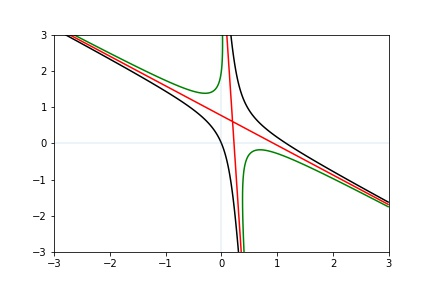
\includegraphics[width=1\columnwidth]{hyperbola.jpg}
\caption{Hyperbola, Asymptotes and Conjugate Hyberbola}
\end{figure}


\end{document}